\documentclass[12pt]{IEEEtran}

\usepackage[utf8]{inputenc}
\usepackage{amsmath}
\usepackage{mathtools}
\usepackage{tcolorbox}

\title{\textbf{Assignment-2}\\ \large AI1110: Probability And Random Variables\\ IIT Hyderabad}
\author{Shivanshu  Ai21btech11027\\ April 11,2022}

\begin{document}
    \maketitle
    \textbf{Q7(b)\hspace{1mm} Evaluate the given finite integral.}
    \[ \int_{-6}^{3} |x+3| \,dx \]
    \textbf{Solution:-}\\
    
    % Redeifination of function
    \begin{equation}
        | x+3 | = 
        \left\{
        \begin{array}{l}
            (x+3)\text{ if }x+3 \geq 0\\
            \vspace{0.01cm} \\
            -(x+3)\text{ if }x+3 < 0\\
        \end{array}
        \right.
    \end{equation}
    \begin{equation}
        | x+3 | = 
        \left\{
        \begin{array}{l}
            (x+3)\text{ if }x \geq -3\\
            \vspace{0.01cm} \\
            -(x+3)\text{ if }x < -3\\
        \end{array}
        \right.
    \end{equation}
    
    % Figure
    \begin{figure}[h]
        \centering
        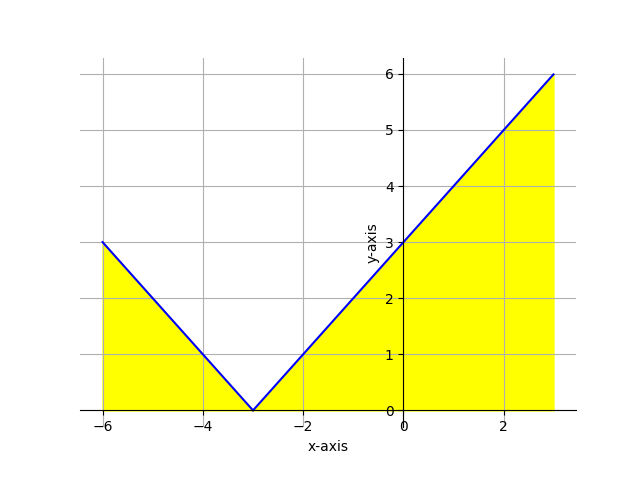
\includegraphics[width=\columnwidth]{Graph.png}
        \caption{Graph of $f(x) = |x+3|$}
        \label{fig.}
    \end{figure}
    
    
     % Box for the identity
    \begin{tcolorbox}
        using the property\\
        \int_{a}^{b} x \,dx = \int_{a}^{c} x \,dx  +  \int_{c}^{b} x \,dx
    \end{tcolorbox}
    
    
    % Starting of proof
    \begin{align}
        I&=\int_{-6}^{3} |x+3| \,dx \\
        &= \int_{-6}^{-3} |x+3| \,dx  +  \int_{-3}^{3} |x+3| \,dx \\
        &= \int_{-6}^{-3} -(x+3) \,dx  +  \int_{-3}^{3} (x+3) \,dx \\
        &= -\left[\frac{x^2}{2}+3x\right]_{-6}^{-3} + \left[\frac{x^2}{2}+3x\right]_{-3}^{3}\\
        &=-\left[\frac{(-3)^2-(-6)^2}{2}+3(-3-(-6))\right]
    \end{align}
    $+\left[\frac{(3)^2-(-3)^2}{2} +3(3-(-6))\right]$
    \begin{align}
        &=-\left[\frac{(9)-(36)}{2} +3(3))\right]
    \end{align}
    $+\left[\frac{(9)-(9)}{2} +3(3))\right]$
    \begin{align}
        &=\frac{27}{2}-9+0+18\\
        &=\frac{27}{2}+9\\
        &=\frac{45}{2}\\
        &=22\frac{1}{2}
    \end{align}
    \implies $ \int_{-6}^{3} |x+3| \,dx $ = $22\frac{1}{2}$ unit.\\
    
\end{document}
